\documentclass[a4j, twocolumn]{jarticle}
% \documentclass[a4j]{jarticle}

\usepackage[dvipdfmx]{graphicx}
\usepackage{subcaption}
\usepackage{caption}

\begin{document}

\title{Queen}
\author{イマム カイリ ルビス\thanks{情報工学分野}}
\date{\today}

\maketitle

\section{クイーンについて}
クイーンは,1970年にロンドンでり結成されたイギリスのロックバンドである.初期の作品はプログレッシブ・ロック,ハード・ロック,ヘヴィ・メタルの影響を受けていたが,次第にアリーナ・ロックやポップ・ロックなどのスタイルを取り入れ,よりコンベンショナルな作品へと変化していった.

\vspace{-5pt}

\begin{itemize}
  \item フレディ・マーキュリー(リードボーカル,ピアノ)
  \item ブライアン・メイ(ギター,ボーカル)
  \item ロジャー・テイラー(ドラム,ボーカル)
  \item ジョン・ディーコン(ベース)
\end{itemize}

\begin{figure}[htb]
  \centering
  \begin{subfigure}[b]{0.15\textwidth}
      \centering
      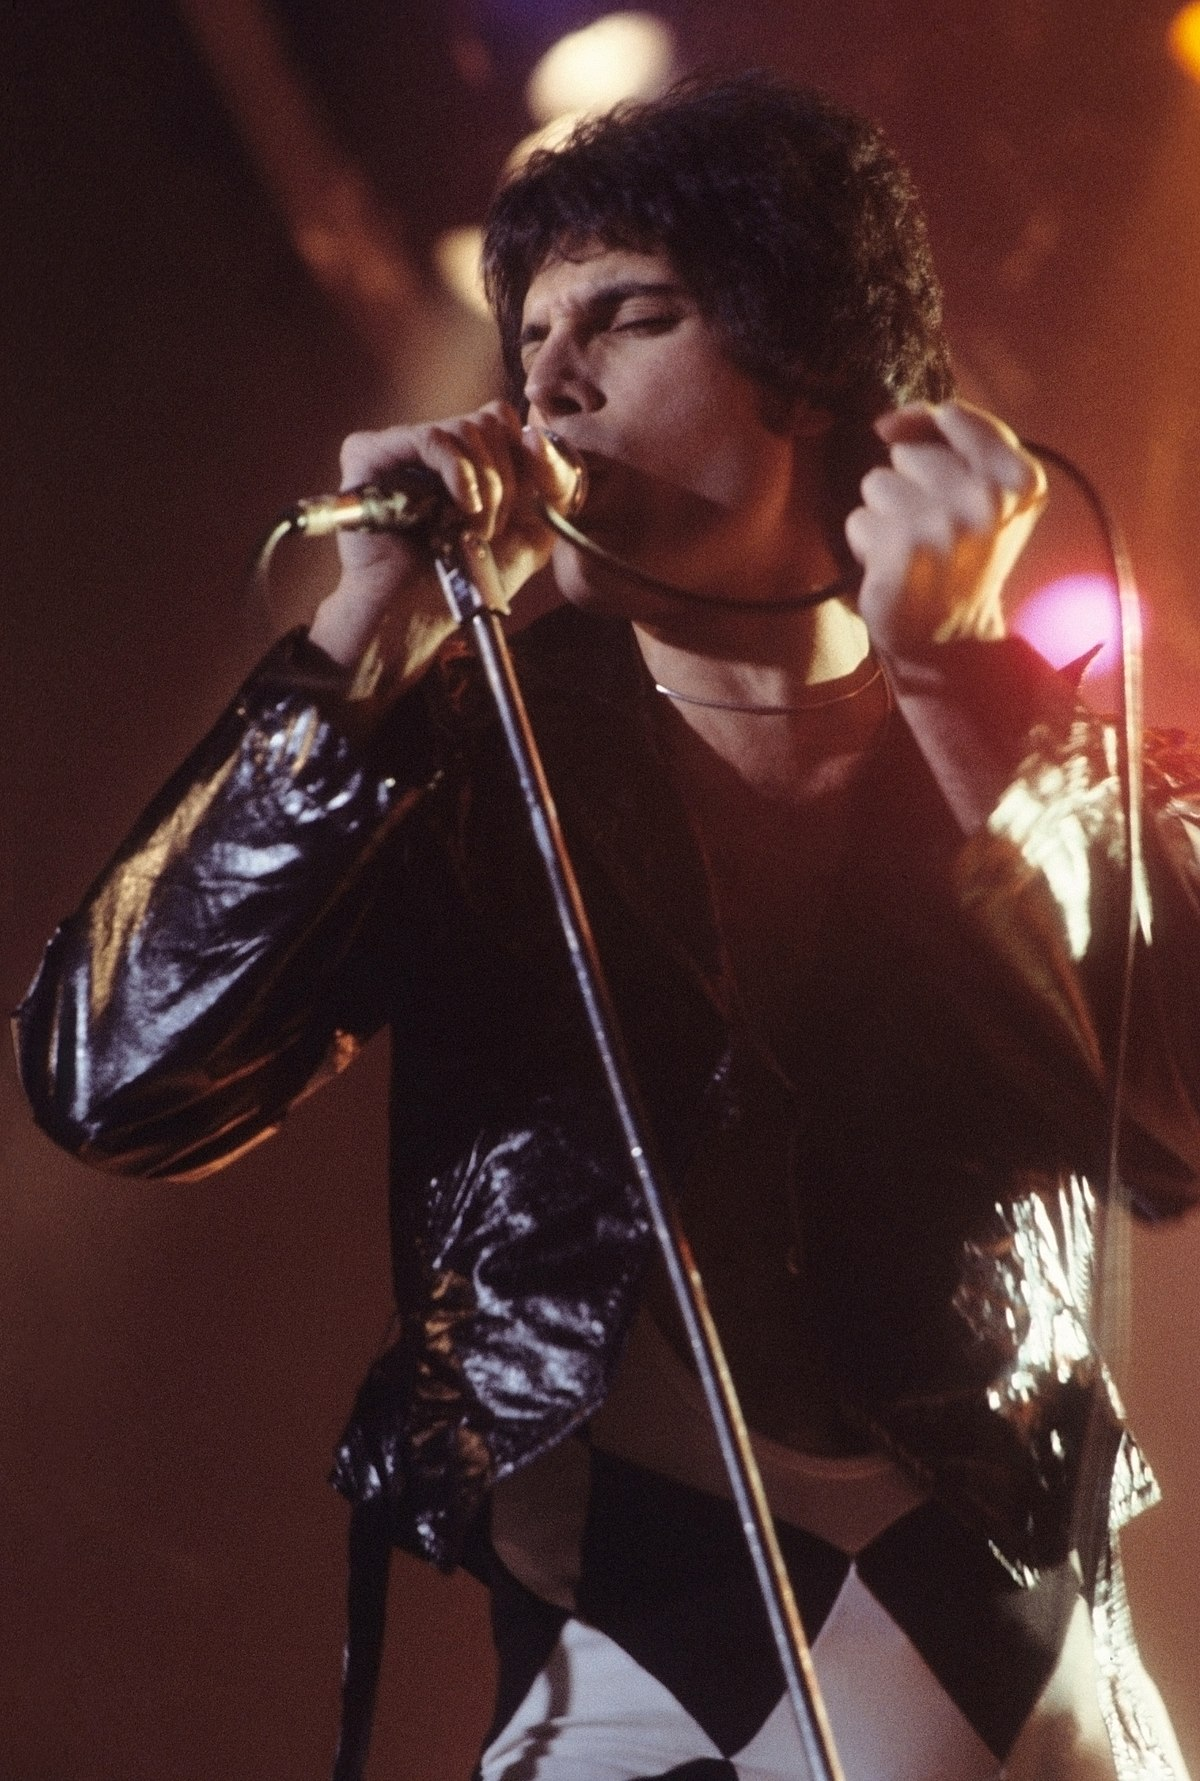
\includegraphics[height=\textwidth]{Freddie.jpg}
      \vspace{-1.0mm}
      \caption{フレディ}
      \label{freddieimg}
  \end{subfigure}
  \begin{subfigure}[b]{0.15\textwidth}
      \centering
      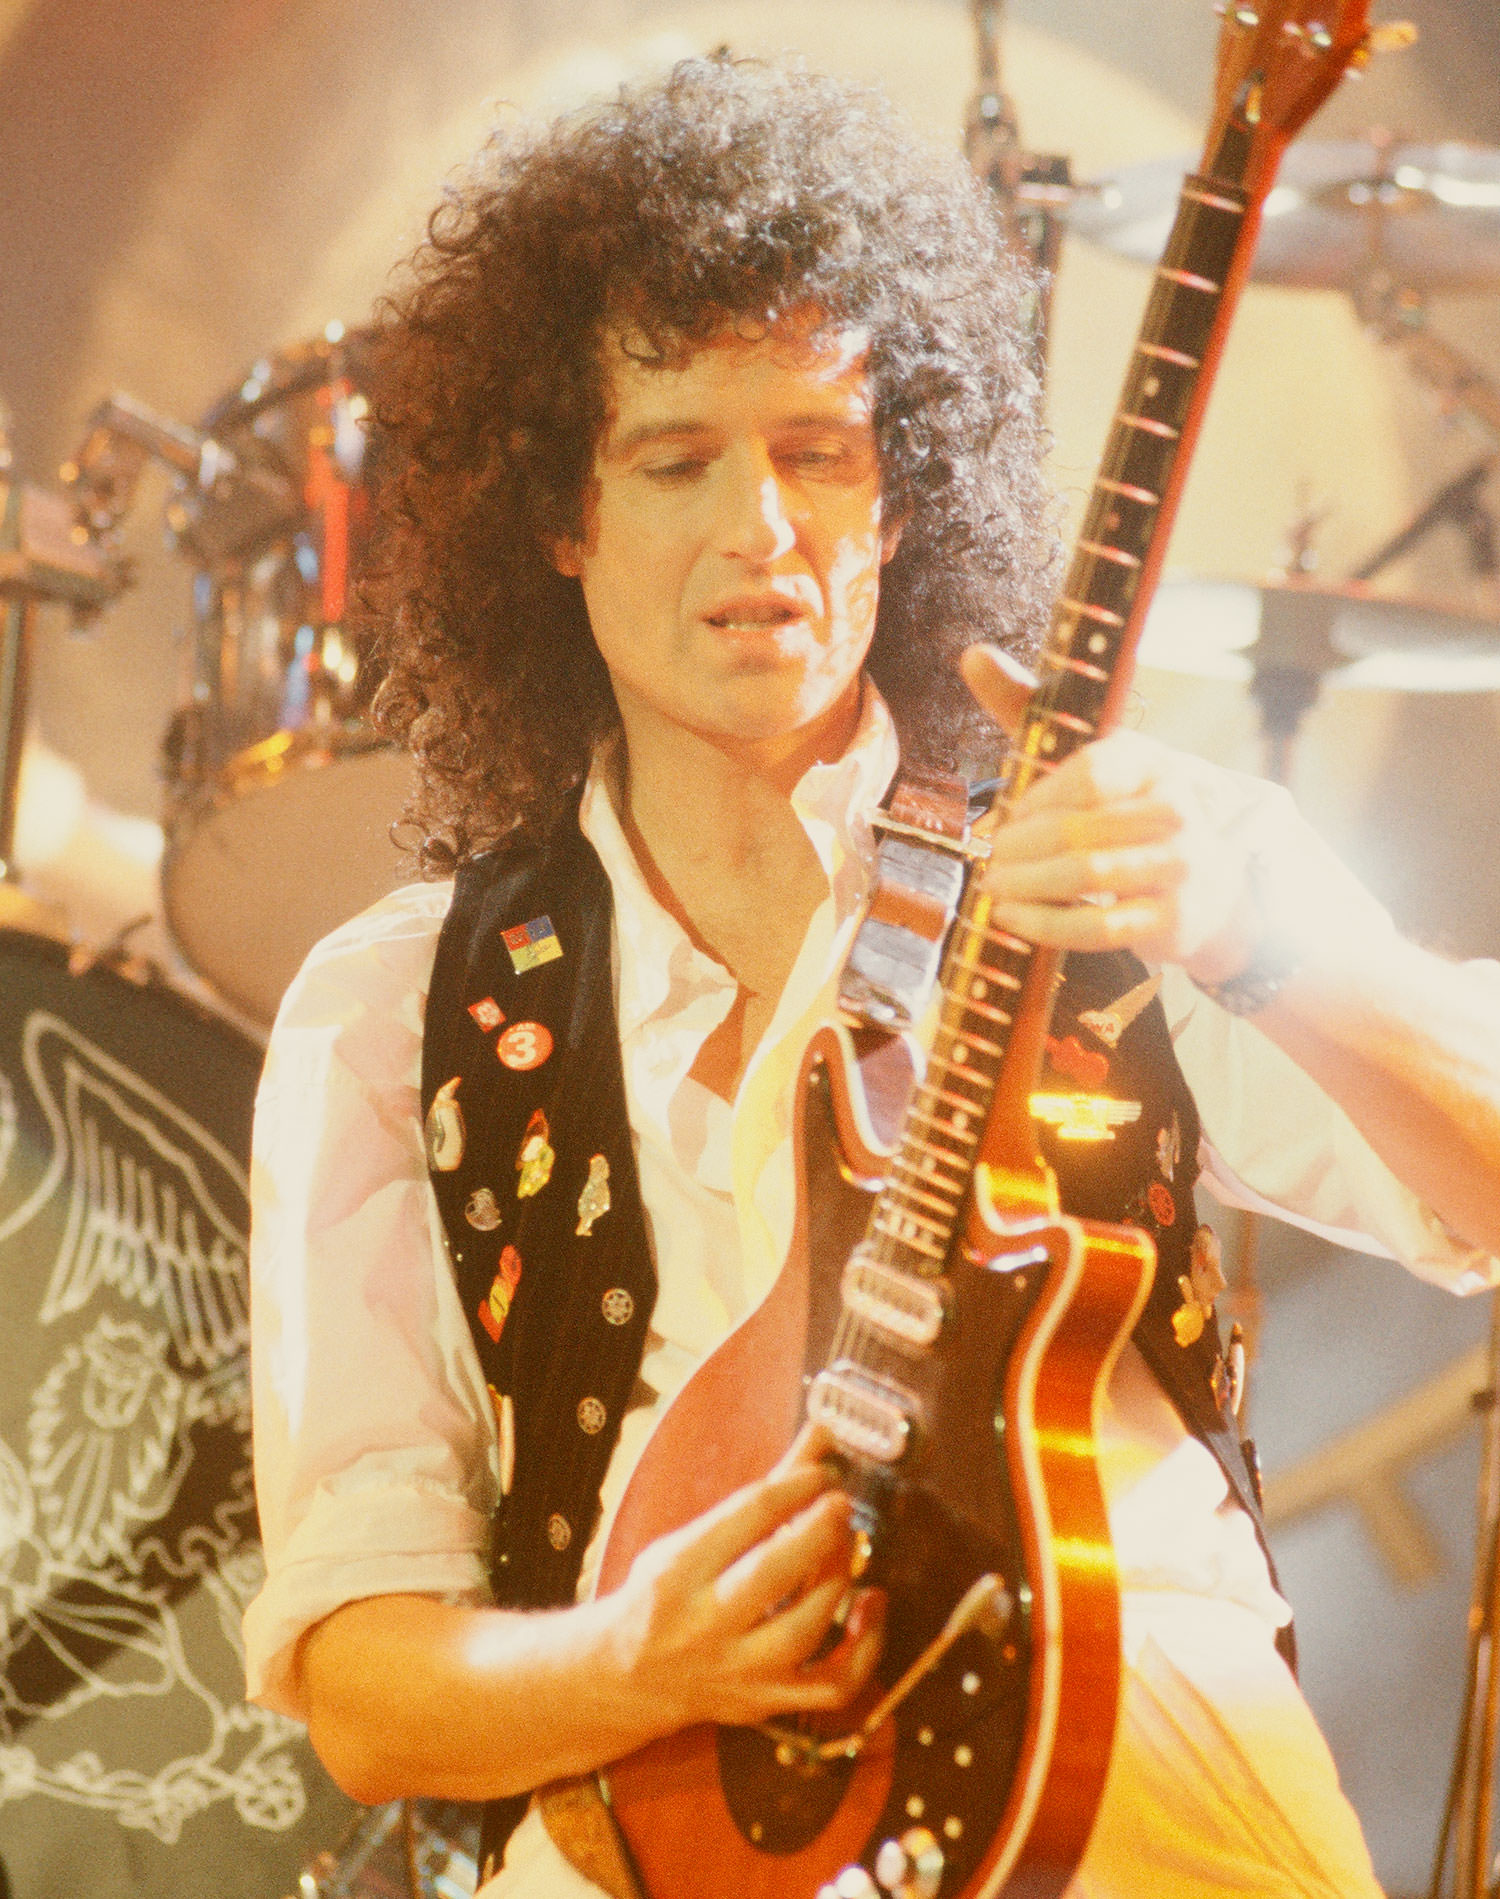
\includegraphics[height=\textwidth]{Brian.jpg}
      \vspace{-1.0mm}
      \caption{ブライアン}
      \label{brianimg}
  \end{subfigure}
  \\
  \begin{subfigure}[b]{0.15\textwidth}
    \centering
    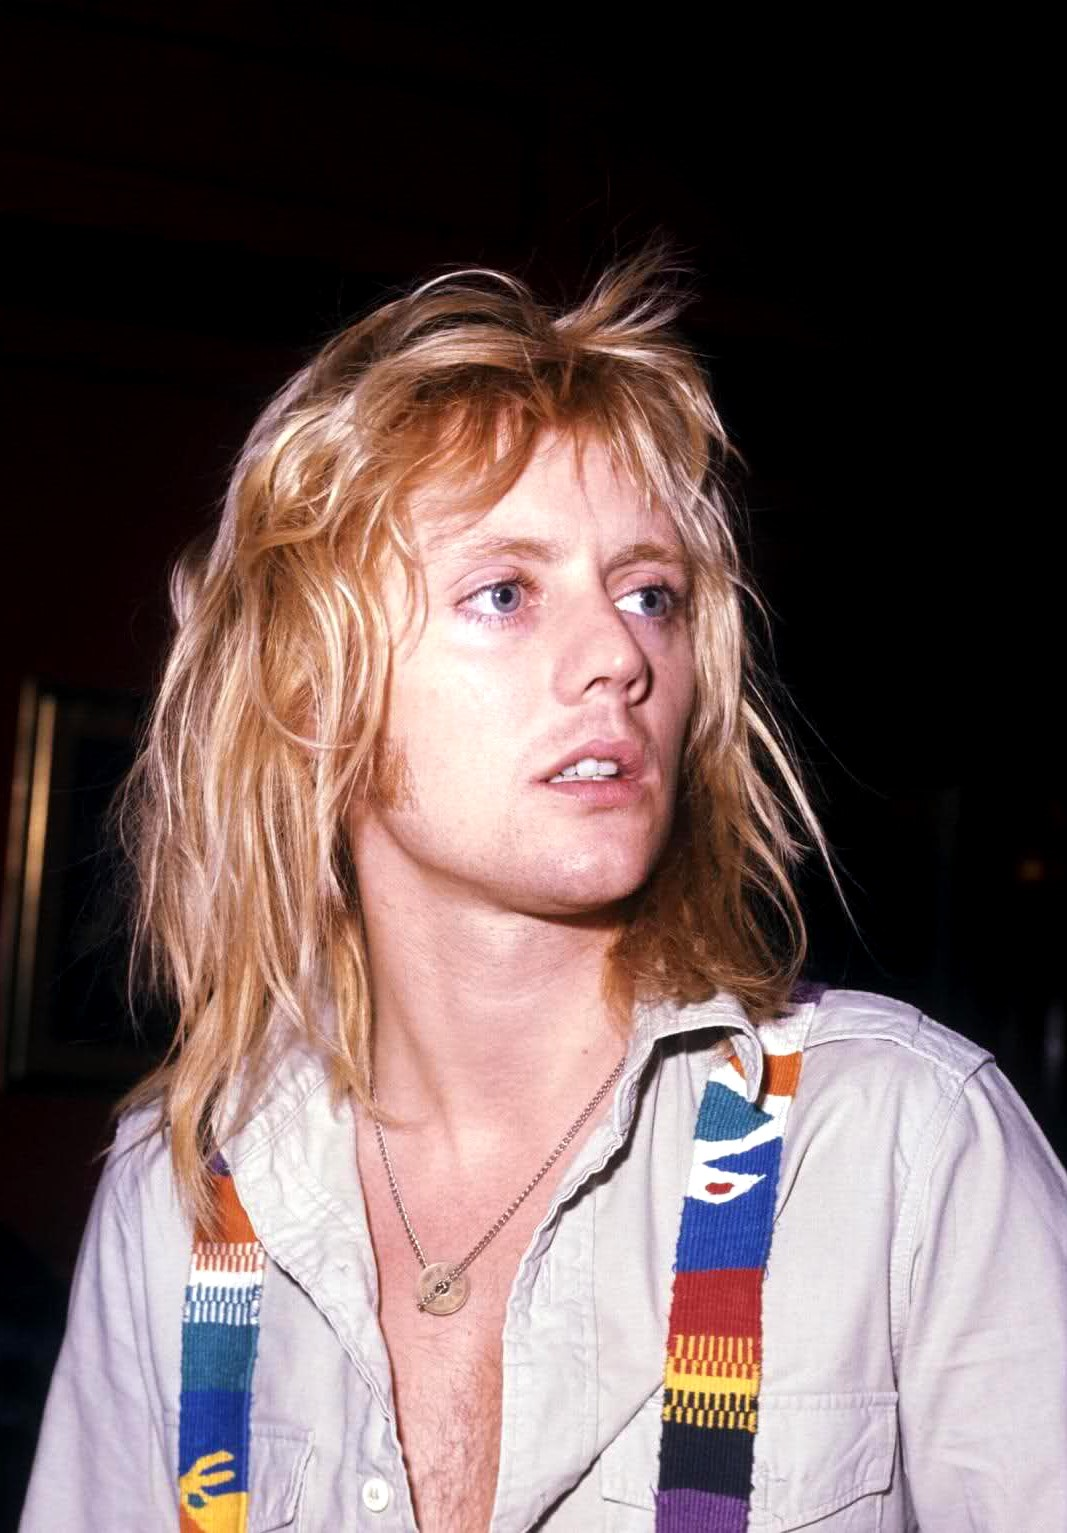
\includegraphics[height=\textwidth]{Roger.jpg}
    \vspace{-1.0mm}
    \caption{フレディ}
    \label{rogerimg}
  \end{subfigure}
  \begin{subfigure}[b]{0.15\textwidth}
    \centering
    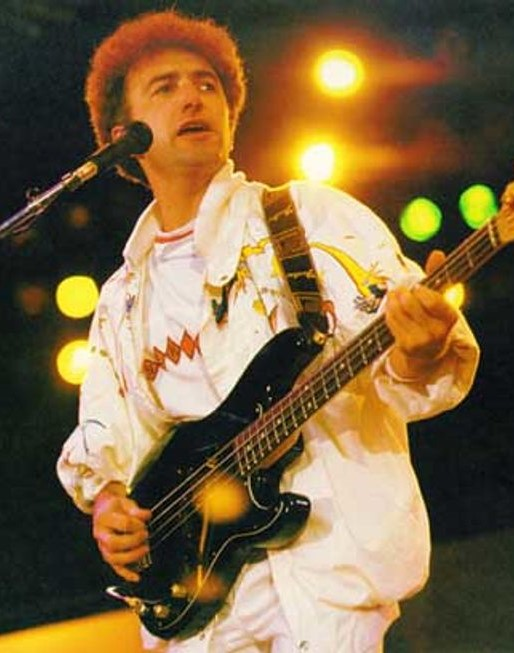
\includegraphics[height=\textwidth]{John.jpg}
    \vspace{-1.0mm}
    \caption{ブライアン}
    \label{johnimg}
  \end{subfigure}
      \vspace{-3.0mm}
      \caption{クイーンのメンバー}
     \label{jpnimg}
\end{figure}

\begin{figure}[htb]
  \begin{center}
      
\includegraphics[scale=0.3]{Queen.jpg}
      \caption{クイーンのロゴ}
      \vspace{-15pt}
      \label{Queen_Image}
  \end{center}
\end{figure}

\vspace{-15pt}

\section{クイーンの誕生}

クイーンの結成メンバーは,1960年代後半に西ロンドンで出会った.ギタリストのブライアン・メイは翌年,ボーカルのティム・スタッフェルと共に1984という名前のグループを結成していた.\cite{Blake}
メイは1968年初頭,インペリアル・カレッジで物理学と赤外線天文学の学位取得に専念するためにグループを脱退し,スタッフェル,キーボーディストのクリス・スミスと「Smile」というグループを結成した.\cite{Blake}

ラインアップを完成するためにメイが大学の掲示板にドラマーを求める広告を出し,若い歯科学生だったロジャー・テイラーがオーディションを受けてこの仕事にありつけた.\cite{Hodkinson}

1970年,スタッフェルはソウルとR\&Bへの興味がグループのハードロックサウンドと衝突すると感じ,成功しないことに嫌気がさしてスマイルを脱退した.\cite{Blake} 残ったメンバーはフレディ・ブルサラをリードボーカルとして受け入れ,テイラーの友人マイク・グローズをベーシストとして採用した.

1971年2月,ジョン・ディーコンがクイーンに加入した.経験豊富なベーシストであることに加え,彼の静かな物腰はバンドを引き立て、エレクトロニクスに長けていた.\cite{Blake}

\section{アルバム}

クイーンは,ハーモニー,複雑なアレンジ,多様なジャンルの音楽など,ユニークな音を持っています.そのため,彼らのアルバムのほとんどは世界中で売れました。

\vspace{-15pt}

\begin{table}[h]
  \caption{アルバムのチャート順位}
  \vspace{-20pt}
  \label{Album_Table}
  \begin{center}
    \begin{tabular}{|c|c|c|c|}
      \hline
                                 &               & \multicolumn{2}{|c|}{順位}\\[0.50ex] \cline{3-4}
      \raisebox{1.5ex}{アルバム名}& \raisebox{1.5ex}{アルバム発売}   
      & UK & JPN\\ [0.50ex] \hline
      Queen                      & 1973年  & 24 & 52\\ \hline
      Queen II                   & 1974年  & 5  & 26\\ \hline
      A Night at the Opera       & 1975年  & 1  & 1 \\ \hline
      A Day at the Races         & 1976年  & 1  & 1 \\ \hline
      News of the World          & 1977年  & 4  & 3 \\ \hline
      Jazz                       & 1978年  & 2  & 5 \\ \hline
    \end{tabular}
  \end{center}
\end{table}

\section{音の強さ}

音響インテンシティは,以下の式から求めることがでる:
\begin{equation}
  \label{eq1}
  I = 
  \frac{
    \Delta p^2
  }{
    2\rho V_w
  }
\end{equation}
圧力変化$\Delta p$, 物質の密度を$\rho$,速さを$V_w$.

ちなみに、ロックコンサートは空間に関係なく,非常に大きな音を出すことができます.平均して,ロックコンサートのデシベルレベルは$90 ~ 120 dB$です.

\section{まとめ}

1991年11月22日にマーキュリーを亡くした後も,クイーンは皆の心の中に特別な位置を占めている.
2002年、クイーンの「ボヘミアン・ラプソディ」は,ギネスワールドレコーズ・ブリティッシュヒットシングルブックが行った投票で,「イギリスで最も好きなヒット曲」に選ばれている.

2004年末,メイとテイラーは、2005年にポール・ロジャース(フリーとバッド・カンパニーの創設者で元リードボーカル)と再結成してツアーに復帰することを発表した.ブライアン・メイのウェブサイトには,ロジャースはマーキュリーの代わりではなく,「クイーン+ポール・ロジャース」としてクイーンと共に「フィーチャー」されるとも書かれていた.引退していたディーコンは参加しなかった.クイーンとポール・ロジャースは2009年5月12日に反目することなく正式に離婚した.

2009年,アメリカン・アイドルの撮影現場で出会ったアダム・ランバートを,クイーンは選びました.彼らは「Queen + Adam Lambert」となり,今日までパフォーマンスを続けています.

\begin{figure}[htb]
  \begin{center}
      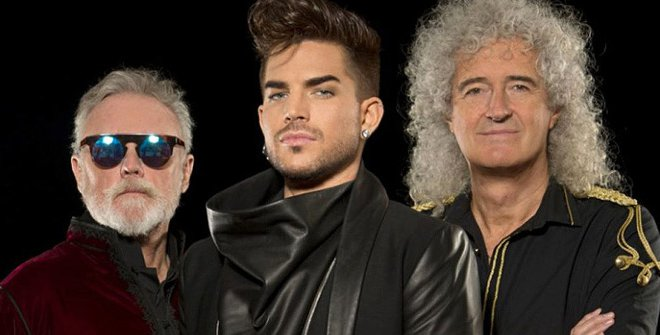
\includegraphics[scale=0.3]{queen_adam_lambert.jpg}
      \caption{Queen + Adam Lambert}
      \vspace{-15pt}
      \label{QueenAdam}
  \end{center}
\end{figure}

\begin{thebibliography}{99}
  \bibitem{Blake}
  Blake, Mark (2016). Freddie Mercury: A Kind of Magic. Omnibus Press.
  \bibitem{Hodkinson}
  Hodkinson, Mark (2004). Queen: The Early Years. London: Music Sales Limited.
\end{thebibliography}
% https://en.wikipedia.org/wiki/Queen_(band)
\end{document}